% Fig 3.2 — MIRACL Arabic dataset structure + evaluation flow

\documentclass[border=4pt]{standalone}
\usepackage{tikz}
\usetikzlibrary{positioning, arrows.meta, shapes.geometric, fit, backgrounds}

\begin{document}
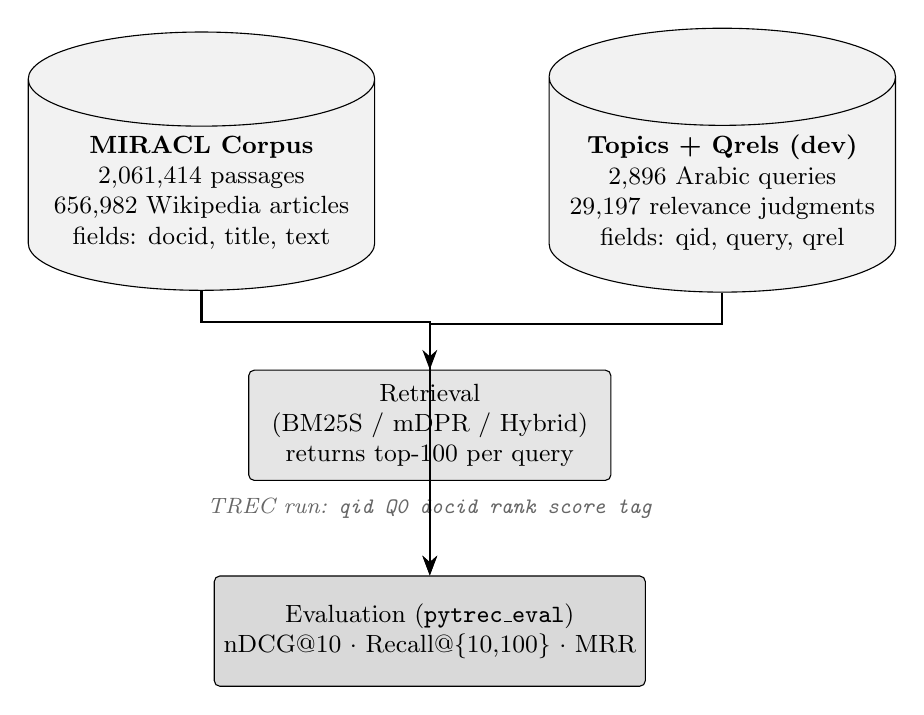
\begin{tikzpicture}[
    >=Stealth,
    node distance=10mm and 14mm,
    box/.style={rectangle, draw, rounded corners=2pt,
                minimum width=46mm, minimum height=14mm,
                align=center, font=\small},
    data/.style={cylinder, shape border rotate=90, aspect=0.3, draw,
                 minimum width=44mm, minimum height=18mm,
                 align=center, font=\small, fill=black!5},
    arrow/.style={-{Stealth[length=2.5mm]}, thick},
    label/.style={font=\footnotesize\itshape, color=black!60}
]
  % Top: two data sources
  \node[data] (corpus) {\textbf{MIRACL Corpus}\\2{,}061{,}414 passages\\656{,}982 Wikipedia articles\\fields: docid, title, text};
  \node[data, right=22mm of corpus] (judg) {\textbf{Topics + Qrels (dev)}\\2{,}896 Arabic queries\\29{,}197 relevance judgments\\fields: qid, query, qrel};

  % Middle: retrieval
  \node[box, fill=black!10, below=of corpus, xshift=29mm] (retr)
    {Retrieval\\(BM25S / mDPR / Hybrid)\\returns top-100 per query};

  % TREC format note
  \node[label, below=1mm of retr]
    {TREC run: \texttt{qid Q0 docid rank score tag}};

  % Bottom: evaluation
  \node[box, fill=black!15, below=12mm of retr] (eval)
    {Evaluation (\texttt{pytrec\_eval})\\nDCG@10 $\cdot$ Recall@\{10,100\} $\cdot$ MRR};

  % Arrows
  \draw[arrow] (corpus.south) -- ++(0, -4mm) -| (retr.north);
  \draw[arrow] (judg.south)   -- ++(0, -4mm) -| (eval.north);
  \draw[arrow] (retr) -- (eval);
\end{tikzpicture}
\end{document}
